\documentclass[american,a4paper,12pt]{article}
\usepackage[T1]{fontenc} %for å bruke æøå
\usepackage[utf8]{inputenc}
\usepackage{graphicx} %for å inkludere grafikk
\usepackage{verbatim} %for å inkludere filer med tegn LaTeX ikke liker
\usepackage{mathpazo}
\usepackage{algorithm} % for algoritmene e.g paragraf 2.2 Gauss
\usepackage{algpseudocode} % lager pseudokode til algoritmene
\usepackage{amsmath}
\usepackage{caption}
\usepackage{multicol}
\usepackage{siunitx}
\usepackage{float}
\usepackage{subcaption}
\usepackage{hyperref}
\hypersetup{
    colorlinks=true,
    linkcolor=black,
    filecolor=magenta,
    urlcolor=blue,
    citecolor=blue
    %pdftitle={Project 1: Computational Physics - FYS3150},
    %pdfpagemode=FullScreen
}

\renewcommand{\vec}[1]{\mathbf{#1}} %ny definisjon av \vec så det blir bold face i stedet for vector-pil.

\captionsetup[table]{skip=10pt}
\bibliographystyle{plain}

\title{Project 1: Computational Physics - FYS3150}
\author{Fredrik Hoftun \& Mikkel Metzsch Jensen}
\date{September 10, 2020}
\begin{document}
\maketitle

\begin{abstract}
  In this project we have looked at three different numerical algorithms for the solving of the one-dimensional Poisson equation with Dirichlet boundary conditions in matrix form. The first two algorithm were based on Gaussian elimination with a forward and backward substitution. The first one were a more general algorithm while the second one was more speliazed for our exact problem. The third algorithm was a LU decomposition of the matrix. We found that the precision of the algorithm increased as $\mathcal{O}(h^2)$ with step size $h \ge \num{e-4}$. At smaller stepsizes the round-off error would dominate giving os best precision for the general algorithm at $h = \num{e-5}$ and the special algorithm at $h \ge \num{e-6}$. We found that the first two algorithms performed similarly regarding CPU time with the special algorithm being 1.5 faster at best. The LU decomposition used considerably more time. This did somewhat reflect on the calculated number of floating point operations for each algorithm which were which were $\mathcal{O}(9n)$, $\mathcal{O}(4n)$ and $\mathcal{O}(2/3\ n^3)$ for general, special, and LU decomposition respectively. 
\end{abstract}
\vfill
\footnotesize{{Link to our GitHub repository: \url{https://github.com/mikkelme/Project_1_FYS3150}}} \newpage

\tableofcontents
\newpage


\section{Introduction}
  In this project we will investegate different algorithms for the solving of the one-dimensional Poisson equation with Dirichlet boundary conditions. This is a problem that is used in many different scientiffic applications. It is used to describe electrostatic and megnetostatic phenonema in a quantitative maner, and it is also helps to understand diffusion and propagation problems. The solution is generally used in a wide range of fields such as engineering, physics, mathematics, biology, chemistry, etc. \cite{poisson_paper}. In this project we have used a second derivative approximation in order to rewrite the problem as a set of linear equations. We have then written three different algorithms: A general and a specialiazed algorithm using gaussian elimination and then one using LU demposition. Theese are described individually in the method sections along with a calculation of the number of floating point operation for each of them. Since we know the analytical solution for our problem we have calculated the relative error for different choices of stepsize $h$ in the algorithm. We have also timed the execution of the algorithms and we compare CPU time of theese computations. We found a significant difference in both precesion and CPU time, which are presented in the results section.
\section{Method}
  \subsection{Defining the problem}
    We are going to solve the one-dimensional Poisson equation with Dirichlet boundary conditions given as follows:
    \begin{align*}
      u''(x) = f(x), \quad x \in (0,1), \quad u(0) = u(1) = 0
    \end{align*}
    In our case we will use the function:
    \begin{align*}
      f(x) = 100e^{-10x}
    \end{align*}
    Note that the algorithms for solving the problem will not be depedent on this specefic choice of f(x). The reason why we stick to this function is for the praticality of having an analytical solution $u(x)$ for f(x):
    \begin{align*}
      u(x) = 1 - (1 - e^{-10})x - e^{-10x}
    \end{align*}
    We can ensure that this is a valid Solution by inserting it into the Poission equation. First we calculate the double derivative of u(x):
    \begin{align*}
      u'(x) = -(1 - e^{-10}) + 10e^{-10x}, \quad u''(x) = -100e^{-10x}
    \end{align*}
    We now see that the solution satisfies the Poisson equation:
    \begin{align*}
      -u''(x) = 100e^{-10x} = f(x)
    \end{align*}
  \subsection{Rewritting the problem as a set of linear equations}
    In order to solve the Poisson equation numerically we discretize $u$ as $v_i$ with $n + 2$ grid points $x_i = ih$ for $i = 0, 1, \hdots, n + 1$. To clarify this gives us a spacing with step length $h = 1/(n + 1)$ and end points $x_0 = 0, \ x_{n+1} = 1$. The boundary conditions is given as $v_0 = v_{n+1} = 0$. We use the following second derivative approximation:
    \begin{center}
      $-u''(x_i) \approx -\frac{v_{i+1} + 2v_i - v_{i+1}}{h^2} =  f(x_i)$ \quad for $i = 1, \hdots, n$
    \end{center}
    $\Longleftrightarrow$
    \begin{align*}
      -v_{i-1} + 2v_i - v_{i+1} = h^2f(x_i)
    \end{align*}
    Notice that we cannot calculate the second derivative approximation at the end points $i = 0$ and $i = n + 1$ since we need to have avaliable points $v_{i \pm 1}$ on either side of $v_i$ for the calculation. We define the colum vector $\vec{v} = [v_1, v_2, \hdots, v_n]$ and try to write out the equation for every step $i = 1, \hdots, n$. As we do this we see a usefull pattern appearing:
    \begin{align*}
          \begin{bmatrix}
            2 & -1 & 0 & \cdots & 0
          \end{bmatrix}
          \begin{bmatrix}
            v_1 \\
            \vdots \\
            v_n
          \end{bmatrix}
    = h^2f(x_1)
    \end{align*}
    \begin{align*}
          \begin{bmatrix}
            2 & -1 & 0 & \cdots & \cdots & 0 \\
            -1 & 2 & -1 & 0 & \cdots & \cdots
          \end{bmatrix}
          \begin{bmatrix}
            v_1 \\
            \vdots \\
            v_n
          \end{bmatrix}
    = h^2
          \begin{bmatrix}
            f(x_1) \\
            f(x_2)
          \end{bmatrix}
    \end{align*}
    \begin{align*}
      \vdots
    \end{align*}
    \begin{align*}
          \begin{bmatrix}
            2 & -1 & 0 & \cdots & \cdots & 0 \\
            -1 & 2 & -1 & 0 & \cdots & \cdots \\
            0 & -1 & 2 & -1 & 0 & \cdots \\
            \cdots & \cdots & \cdots & \cdots & \cdots & \cdots \\
            0 & \cdots & & -1 & 2 & -1 \\
            0 & \cdots & & 0 & -1 & 2
          \end{bmatrix}
          \begin{bmatrix}
            v_1 \\
            \vdots \\
            v_n
          \end{bmatrix}
    = h^2
          \begin{bmatrix}
            f(x_1) \\
            f(x_2) \\
            \vdots \\
            f_n
          \end{bmatrix}
    \end{align*}
    \\ From this we see that we can write the problem as a set of linear equation using a matrix $\vec{A}$:
    \begin{align*}
      \vec{A}\vec{v} = \vec{g}
    \end{align*}
    With the following definitions:\\
    \begin{align*}
      \vec{A} =
      \begin{bmatrix}
        2 & -1 & 0 & \cdots & \cdots & 0 \\
        -1 & 2 & -1 & 0 & \cdots & \cdots \\
        0 & -1 & 2 & -1 & 0 & \cdots \\
        \cdots & \cdots & \cdots & \cdots & \cdots & \cdots \\
        0 & \cdots & & -1 & 2 & -1 \\
        0 & \cdots & & 0 & -1 & 2
      \end{bmatrix}
      \quad, \vec{v} =
      \begin{bmatrix}
        v_1 \\
        v_2 \\
        \vdots \\
        v_n
      \end{bmatrix}
      \quad, \vec{\tilde{g}} = h^2
      \begin{bmatrix}
        f(x_1) \\
        f(x_2) \\
        \vdots \\
        f_n
      \end{bmatrix}
    \end{align*}
\subsection{General solution using Gausian elimination}
We can solve our set of linear equations using Gaussian elimination on the matrix $\vec{A}\vec{v} = \vec{g}$. In the beginning we assume a more generilazed matrix $\vec{A}$ as:
\begin{align*}
  A =
  \begin{bmatrix}
    b_1 & c_1 & 0 & \cdots & \cdots & 0 \\
    a_1 & b_2 & c_2 & 0 & \cdots & \cdots \\
    0 & a_2 & b_3 & c_3 & 0 & \cdots \\
    \cdots & \cdots & \cdots & \cdots & \cdots & \cdots \\
    0 & \cdots & & a_{n-2} & b_{n-1} & c_{n-1} \\
    0 & \cdots & & 0 & a_{n-1} & b_n
  \end{bmatrix}
\end{align*}
\\ Here $a_i$ are the elements below the diagonal, $b_i$ are the elements on the diagonal and $c_i$ are the elements above the diagonal. In order to solve this we use first a forward substitution and then a backwards substitution \cite{linalg}. The implementation of this is showed in Algorithm 1:
\begin{algorithm}[H]
\caption{General algorithm}
\begin{algorithmic}[1] %fra algpseudocode
  \For {$i = 2, \dots, n$} \Comment{Forward substitution eliminating $a_i$}
    \State $b_i = b_i - c_{i-1}\cdot {a_i}/{{b}_{i-1}}$ \Comment{Update ${b}_i$}
    \State $g_i = g_i - {g}_{i-1}\cdot {a_i}/{{b}_{i-1}}$ \Comment{Update ${g}_i$}
  \EndFor
  \Statex
  \State $v_0 = v_{n+1} = 0$ \Comment{Backward substitution obtaining $v_i$}
  \State $v_n = g_n/B_n;$
  \For {$i = n-1, \dots, 1$}
    \State $v_i = (g_i - c_i\cdot v_{i+1})/b_i$ % \frac{g_i - c_i\cdot v_{i+1}}{b_i}$
  \EndFor
\end{algorithmic}
\end{algorithm}
By running this algorithm for decreasing step length we se that the numerical solution aproaches the analytical quite fast (see figure \ref{fig:general_ex})
\begin{figure}[H]
\begin{center}
  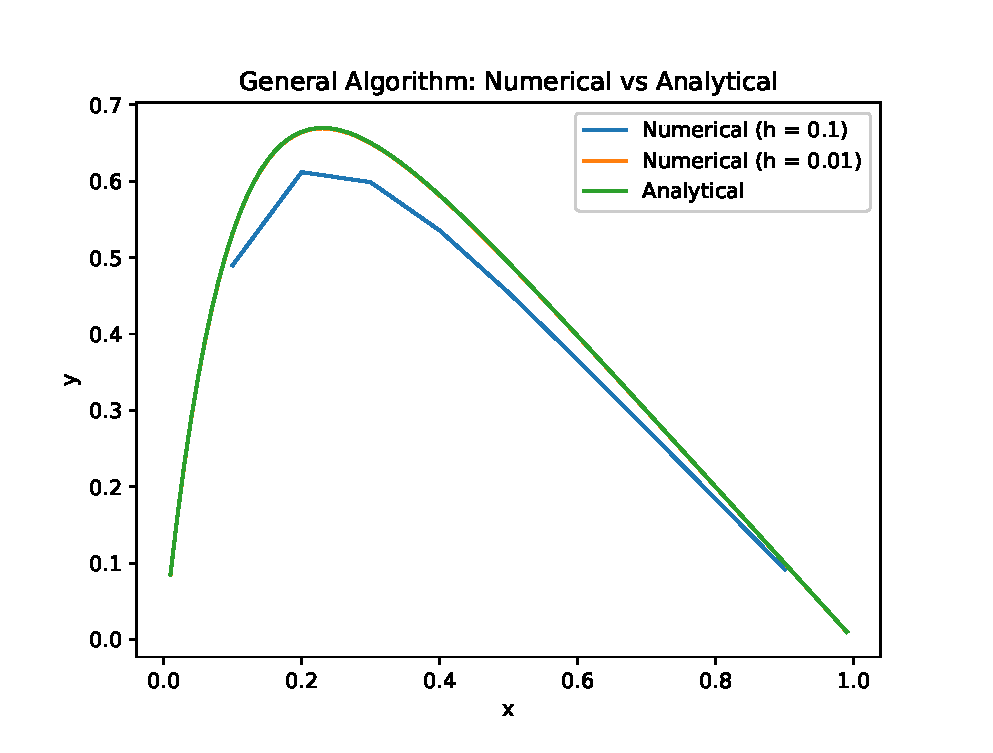
\includegraphics[width = \textwidth]{figures/general_algo_example.eps} \\
  \caption{The figure shows the analytical solution and the numerical solution using the generel algorithm for $h = 0.1$ and $h = 0.01$ respectively. We see that the numerical solution lines up with the analytical solution already for $h = 0.01$.}
  \label{fig:general_ex}
  \end{center}
\end{figure}
We can calculate the algorithms number of Floating Point Operations. In our forward substitution we have $2 \cdot 3$ operations for each loop which runs for a total of $n-1$ times. In the backward substitution we have a single leading operation and then 3 operations which also loops for a total of $n-1$. The total number of the operations is then
\begin{align*}
  (6 + 3)(n - 1) + 1 = 9n - 8
\end{align*}
For large n we can approximate this as 9n.
\subsection{Simplified specific solution}
Since we actually have the fixed values $a_i = -1,\ b_i = 2,\ c_i = -1$ for all i for the matrix $\vec{A}$, we can simplify our algorithm even more. Now we can do the forward substitution before hand:
\begin{align*}
    \vec{A} =
    \begin{bmatrix}
    2 & -1 & 0 & \cdots & \cdots & 0 \\
    -1 & 2 & -1 & 0 & \cdots & \cdots \\
    0 & -1 & 2 & -1 & 0 & \cdots \\
    \cdots & \cdots & \cdots & \cdots & \cdots & \cdots \\
    0 & \cdots & & -1 & 2 & -1 \\
    0 & \cdots & & 0 & -1 & 2
    \end{bmatrix}
    \ \sim \
    \begin{bmatrix}
    2 & -1 & 0 & \cdots & \cdots & 0 \\
    0 & 3/2 & -1 & 0 & \cdots & \cdots \\
    0 & -1 & 2 & -1 & 0 & \cdots \\
    \cdots & \cdots & \cdots & \cdots & \cdots & \cdots \\
    0 & \cdots & & -1 & 2 & -1 \\
    0 & \cdots & & 0 & -1 & 2
    \end{bmatrix}
\end{align*}
\begin{align*}
    \quad \sim
    \begin{bmatrix}
    2 & -1 & 0 & \cdots & \cdots & 0 \\
    0 & 3/2 & -1 & 0 & \cdots & \cdots \\
    0 & 0 & 4/3 & -1 & 0 & \cdots \\
    \cdots & \cdots & \cdots & \cdots & \cdots & \cdots \\
    0 & \cdots & & -1 & 2 & -1 \\
    0 & \cdots & & 0 & -1 & 2
    \end{bmatrix}
    \ \sim \
    \begin{bmatrix}
    2 & -1 & 0 & \cdots & \cdots & 0 \\
    0 & 3/2 & -1 & 0 & \cdots & \cdots \\
    0 & 0 & 4/3 & -1 & 0 & \cdots \\
    \cdots & \cdots & \cdots & \cdots & \cdots & \cdots \\
    0 & \cdots & & 0 & i_n/{i_n-1} & -1 \\
    0 & \cdots & & 0 & 0 & {i_n+1}/i_n
    \end{bmatrix} \\
\end{align*}
We see that the updated diagonal element $b_i$ follows the formula:
\begin{align*}
   b_i = \frac{i+1}{i}
\end{align*}
This means that the update of the diagonal element now use 2 floating point operations per n (1 less than before), but more important this can be precalculated and in practice excluded from the algorithm. We can therefore justify not to count theese floating point operations. The update of $g_i$ with known values for a, b and c simplifies to:
\begin{align*}
  g_i = g_i + g_{i-1}/{b_{i-1}}
\end{align*}
\cite{linalg}. This gives us the following special algorithm:
\begin{algorithm}[H]
\caption{Special algorithm, where $a_i = -1,\ b_i = 2,\ c_i = -1$}
\begin{algorithmic}[1]
  \For {$i = 1, \dots, n$} \Comment{Pre-calculating $b_i$}
    \State $b_i = {i+1}/i$
  \EndFor
  \Statex
  \For {$i = 2, \dots, n$} \Comment{Forward substitution eliminating $a_i$}
    \State $g_i = g_i + g_{i-1}/{b_{i-1}}$ \Comment{Update $g_i$}
  \EndFor
  \Statex
  \State $v_n = 0$ \Comment{Backward substitution obtaining $v_i$}
  \For {$i = n-1, \dots, 1$}
    \State $v_i = \frac{g_i + v_{i+1}}{b_i}$
  \EndFor
\end{algorithmic}
\end{algorithm}
Similarly to the general algorithm we can calculate the total number of floating point operations (not including calculation of $b_i$):
\begin{align*}
  (2 + 2)(n-2) = 4n - 8
\end{align*}
For large n this can be approximated to $4n$. When running the script with this algorithm we see indically results for $h= 0.1$ and $h=0.01$ (see figure \ref{fig:special_ex}) as we did with the gerneral algorithm.
\begin{figure}[H]
\begin{center}
  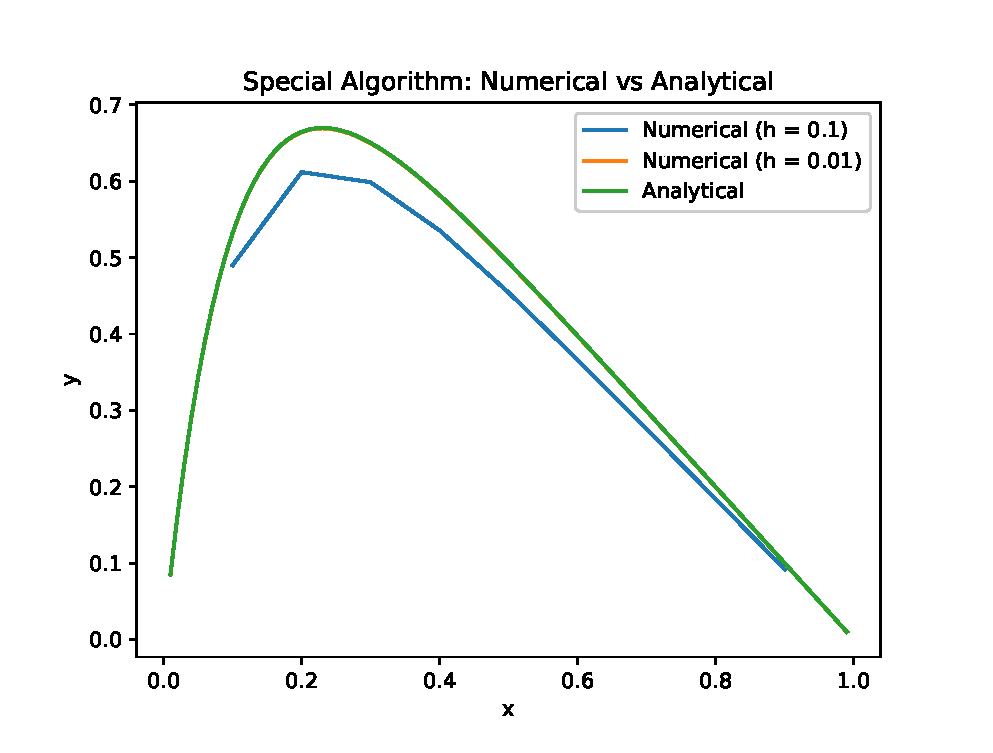
\includegraphics[width = \textwidth]{figures/special_algo_example.eps} \\
  \caption{The figure shows the analytical solution and the numerical solution using the special algorithm for $h = 0.1$ and $h = 0.01$ respectively. We see that the numerical solution lines up with the analytical solution already for $h = 0.01$.}
  \label{fig:special_ex}
  \end{center}
\end{figure}
\subsection{LU decomposition}
For the LU decomposition we have our triangular matrix $\vec{A}$ which can be divided into two invertible matrices, consisting of one upper triangular matrix $\vec{U}$ and one lower triangular matrix $\vec{L}$. We then get the LU decomposition:
\begin{align*}
    \vec{Av} &= \vec{g} = \vec{LUv}\\
    \vec{Uv} &= \vec{L^{-1}g = \vec{w}}
\end{align*}
The Armadillo \cite{Armadillo} library for \verb!C++! allows for easy computation of the matrices.\\
The LU decomposition uses $\mathcal{O}(2/3\ n^3)$ FLOPS for the computation, making it much heavier than the general and special algorithms.

\subsubsection*{Proof that L or U is invertible}
A matrix is invertible if the determinant is not equal to zero; $\det A \neq 0$. A property of triangular matrices is that the determinant is the product of the values on the diagonal. In our case we have non-zero real numbers so the matrices are invertible.

\subsubsection*{Memory use}
Since we need to define the whole matrix when using LU decompoistion it becomes more heavy one the Random Acces Memory (RAM). When defining a $n \times n$ matrix with double precision (64 bits) we use a total amount of memory storage:
\begin{align*}
  \text{memory needed} = n^2 \cdot64 \ \text{bits} = n^2 \cdot 8 \ \text{bytes}
\end{align*}
We see that the memory needed grows quite fast when increasing n by 10:
\begin{table}[H]
  \begin{center}
  \caption{Memory (RAM) needed for a $n \times n$ matrix}
  \begin{tabular}{|c|c|c|c|} \hline
  \textbf{n} & \textbf{Memory needed} \\ \hline
  $10^1$ & 800 B \\ \hline
  $10^2$ & 80 kB \\ \hline
  $10^3$ & 8 mB \\ \hline
  $10^4$ & 800 mB \\ \hline
  $10^5$ & 80 GB \\ \hline
  \end{tabular}
  \end{center}
  \label{tab:RAM}
\end{table}
The machine that we are using have 4 GB of RAM and therefore we cannot initialize a $\num{e5} \times \num{e5}$ matrix.
\subsection{Comparing precision and time}
In order to compare the precesion of the different algorithms we will use the relative error between the numerical solution ($v_i$) and the analytical solution ($f(x_i)$). For practical reasons we will use the base 10 logarithm so the relative error is given as
\begin{align*}
  \epsilon_i = log_{10}\left|\frac{v_i - u_i}{u_i}\right|
\end{align*}
Since we divide with the analytical solution $u_i$ in this expression we cannot make the calculation for the end points where $u_0 = u_{n+1} = 0$. This means that we will only calculate $\epsilon_i$ for $i = 1, \hdots, n$. When we lower the step length $h$ we expect the error to decrease as well. When plotting $h$ with a logaritmic axis (base 10) against $\epsilon_i$ we should see a linear trend. The slope of this trend can then be usefull in order determain the relationship between step length and precesion. At some point though we could expect this trend to interrupted by erros due round-off. We want to investegate if and when this happens.\\
In addition we will also investegate whether we see any different in CPU time between the different algorithms. We expect that the timing will reflect back on the number of floating point operations done in each algorithm.
\subsection{Implementation}
We used \verb!C++! to implement our algorithms. The results from \verb!C++! scripts a written to text file and then manage in python for plotting and presentation of the results.
\section{Results}
  We collected the maximum of the relative error $\epsilon$ for all the three algorithms for different values for the step length $h$. The result is shown in figure \ref{fig:max_err}.
  \begin{figure}[H]
  \begin{center}
    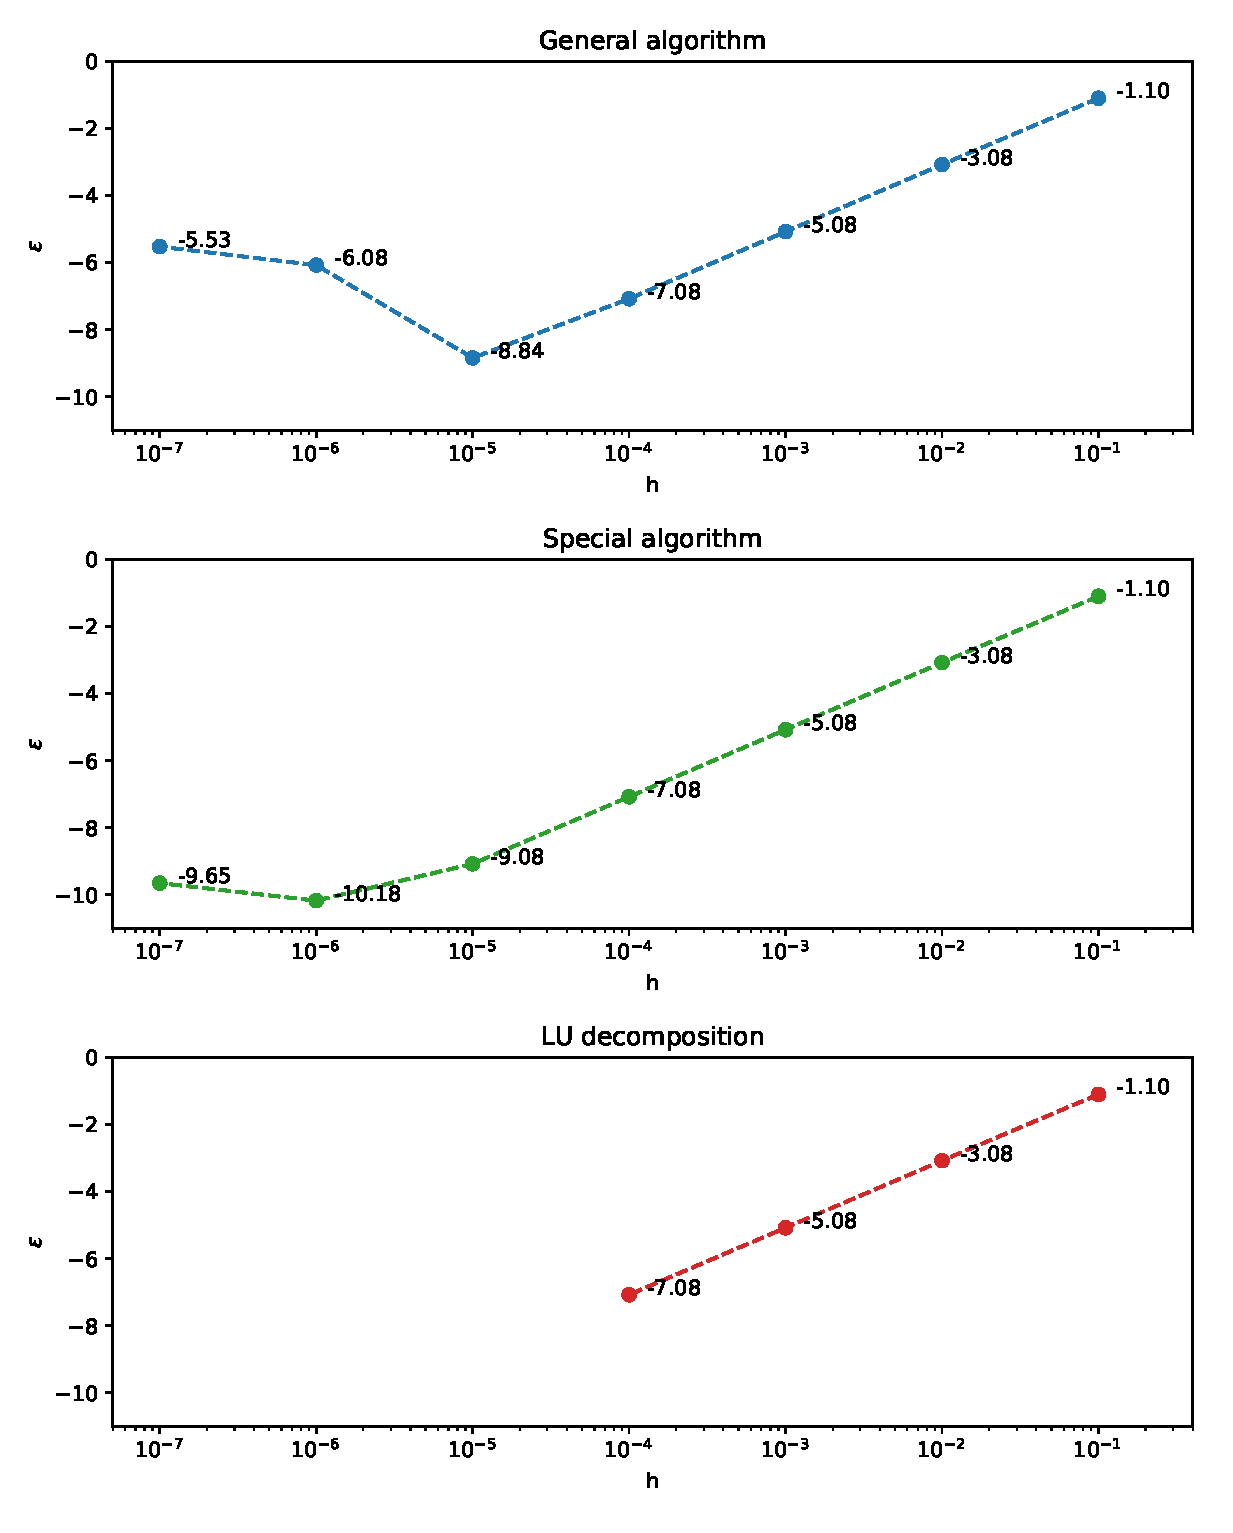
\includegraphics[width = \textwidth]{figures/max_err.eps} \\
    \caption{Relative error $\epsilon$ for different step length $h$ for the three diferent algorithms. Note that relative error is defined with a logarithm and h is also plotted on a logaritmic axis.}
    \label{fig:max_err}
    \end{center}
  \end{figure}
  Note that we were not able to produce the results for LU decompositions with $h \le \num{e-5}$ because we did not have enough memory to store a matrix of size $\num{e5} \times \num{e5}$ or larger. \\
  The CPU time for the execution of the different runs can be seen in table \ref{tab:final_res}. Note that this varied a lot between each repetition of measurements, and it might therefore not be very reliable for small comparisons.
  \begin{table}[H]
    \begin{center}
    \caption{CPU Time for the execution of the algorithms for diffrent choices of n, where n is the number of steps. Recall that we have $n \propto h^{-1}$}
    \begin{tabular}{|c|c|c|c|} \hline
    \textbf{n} & \textbf{General algorithm: t [s]} & \textbf{Special algorithm: t [s]} & \textbf{LU Decomposition: t [s]} \\ \hline
    $10^1$ & $\num{3e-6}$     & $\num{2e-6}$    & $\num{9.81e-4}$ \\ \hline
    $10^2$ & $\num{4e-6}$     & $\num{4e-6}$    & $\num{1.96e-4}$ \\ \hline
    $10^3$ & $\num{3.8e-5}$   & $\num{3.2e-5}$  & $\num{1.02e-2}$ \\ \hline
    $10^4$ & $\num{3.41e-4}$  & $\num{3.42e-4}$ & $\num{2.45e0}$ \\ \hline
    $10^5$ & $\num{3.79e-3}$  & $\num{2.35e-3}$ & nan \\ \hline
    $10^6$ & $\num{3.57e-2}$  & $\num{2.38e-2}$ & nan \\ \hline
    $10^7$ & $\num{3.16e-1}$  & $\num{2.26e-1}$ & nan \\ \hline
    \end{tabular}
    \label{tab:final_res}
    \end{center}
  \end{table}
  The computer which we ran all the programs have the following specs:
  \begin{align*}
    \text{CPU} &= \text{2.5 GHz Intel Core i5} \\
    \text{RAM} &= \text{4 GB 1333 MHz DDR3}
  \end{align*}
\section{Discussion}
Regarding the development of the maximum relative error (showed in figure \ref{fig:max_err}) we saw the expected trend that we were looking for. For all the algorithms we got a linear connection between $log_{10}(h)$ and $\epsilon$ for $h \ge \num{e-4}$. In this interval $\epsilon$ drops about 2 points for each logarithmic decreasement in h. This tell us that the error is proportional to $h^2$:
\begin{align*}
  \epsilon = \mathcal{O}(h^2)
\end{align*}
From the results we also see that the linear trend is broken at some point given us a point of minimum error. Since we were not able to go lower than $h = \num{-4}$ for the LU decomposition we can only compare the general and special algorithm here. In both theese cases the linear trend is broken around $h = \num{-5}$. For the general algorithm this happens quite drastically leaving us with a minimum relative error of -8.84. For the special algorithm the error keeps decreasing all the way down to -10.18 at $h = \num{-6}$. This loss of precision happens due to round-off erros when we are handling too many small calculations. In the case of the special algorithm we see that the simplified algorithm with fewer calculations make us able to archieve higher precesion. If we had to extract the most reliable solution from this problem we should choose to run the special algorithm with $h \approx \num{-6}$. This might not be the precise minimum point, and we could still vary $h$ in even smaller increaments to check for lower relative errors. \\
Regarding the CPU time we got some mixed results. First of all we expected that the number of floating point operations would be proportional to the CPU time. Recall that we found the following relation for the floating point operations:
\begin{align*}
  \text{General algorithm} &= \mathcal{O}(9n) \\
  \text{Special algorithm} &= \mathcal{O}(4n) \\
  \text{LU decompoistion} &= \mathcal{O}(2/3\ n^3) \\
\end{align*}
We see that increasements in $n$ by the order of 10 also produces increasements in CPU time for the general end special algorithm by 10, just as expected. This does not hold true for the transistion from $n = 10$ to $n = 100$ but we will se past this since the short computation time might make these results more uncertain here. For the LU decomposition we expected to se an increasement in CPU time with a factor of $\nume{e3}$ for each time, but we saw it increase with a factor of $\nume{e2}$. We later found that the armadillo solver might have used a more clever approach to this problem. On the documentation it says that the solver can use different solving techniques if it recognize that the problem can be simplified: "By default, matrix A is analysed to automatically determine whether it is a general matrix, band matrix, diagonal matrix, or symmetric/hermitian positive definite (SPD) matrix; based on the detected matrix structure, a specialised solver is used for faster execution" \cite{Armadillo}. Therefore we can not use this a reliable example of LU decompoistion. Regarding the difference CPU time between the general and special algorithm we expected the time difference to be $\frac{9n}{4n} = 2.25$. The results showed that the special algorithm was somewhat faster at large n. For n = $\num{e6}$ we had a difference of:
\begin{align*}
  \frac{\num{3.57e-2}}{\num{2.38e-2}} = 1.5
\end{align*}
This is not quite as fast as expected though. We do not have any certain explanation for this, but we cannot make any conclusion without having a mean timing for mutiple runs.\\
Anyway by using the calculated number of operations for each algorithm and the timing we can check whether this comes close the number of FLOPS (Floating Point Operations Per Second) that the CPU should be able to perfom. This computer should be able to make a maximum of $\num2.5e9$ FLOPS. We can inevestegate the number of FLOPS for the general algorithm with $n = \num{e7}$:
\begin{center}
  $FP = \num{9e7} - 17 \approx \num{9e7}$
\end{center}
\begin{center}
  $\text{CPU Time} = 0.316 \ s$
\end{center}
\begin{center}
  FLOPS = FP / CPU Time $\approx 0.28 \ GHz$
\end{center}
We see that there are some room up the maximum capacity of the processor (2.5 GHz), but this might be somewhat expectable. Remember that we did not take any other operation into account, such as writting and reading from memory.
\section{Conclusion}
In this report we have used three different ways of solving the one-dimensional Poisson equation with Dirichlet boundary conditions in matrix form and have seen that efficiency of the methods vary greatly. First of all we saw that precesion of the algorithms increased as $\mathcal{O}(h^2)$ with step size $h \ge \num{e-4}$. For smaller stepsizes we found that the precesion was affected by round-off errors. This lead to the general algorithm having the best precision at $h = \num{e-5}$ and the special algorithm having the best precision at $h \ge \num{e-6}$. We were not able to make this kind of conclusions on the LU decompoistion method because of memory lack. The general and special algorithms were comparable in computation time with the special algorithm being around 1.5 time faster than the general, while the LU decomposition lagged greatly behind. This were somewhat relatable to the number of floating point operations for each algorithms which were $\mathcal{O}(9n)$, $\mathcal{O}(4n)$ and $\mathcal{O}(2/3\ n^3)$ for general, special, and LU decomposition respectively. We have learned the importance of choosing the correct algorithm, and that specialising it will make for some more efficient and accurate code.


\begin{thebibliography}{9}
  \bibitem{poisson_paper} S. B. Gueye, K. Talla and C. Mbow, "Solution of 1d poisson equation with neumann-dirichlet and dirichlet-neumann boundary conditions using the finite difference method", Journal of Electromagnetic Analysis and Applications, Vol. 6, No. 10, pp. 309, 2014.

  \bibitem{linalg} Hjort-Jensen, M., 2018. Computational Physics Lectures: Linear Algebra methods,  accesable at course github repository. \url{http://compphysics.github.io/ComputationalPhysics/doc/pub/linalg/pdf/linalg-print.pdf}

  \bibitem{Armadillo} Armadillo's website: \url{http://arma.sourceforge.net/}


\end{thebibliography}
\section*{Appendix}
GitHub repository: \url{https://github.com/mikkelme/Project_1_FYS3150}



%It is possible in Unix systems to run scripts in for loops. Use the command \emph{for i in \{1..N\}; do %PATH; done > filename.txt} e.g. for a file general in the directory general\_solution do with N = 10 and %$10^n$ = 4\ do: \emph{for i in \{1..10\};do ./general\_solution/general 4; done > filename.txt}. This %will run the file general 10 times with n = 4.


\end{document}
